\chapter{Solving differential equations}

Before you start talking about solving a single partial differential equation (PDE) or PDE system, as well as about neural networks, you need to clearly understand what methods exist to solve this problem, how they work, what strengths and weaknesses, what facts affect quality decision. After that, you also need to understand how regression models are constructed, evaluated, and explained. Thus, starting with the simplest linear regression model, results will be obtained that will allow us to construct good approximations based on Fourier or Chebyshev series from the available data or the available quality function. One of the most important results related to the approximation of functions is a model of artificial neural networks based on a sigmoid function. Tsybenko’s theorem guarantees the convergence of model parameters to the desired function with arbitrary accuracy, for example. When considering differential equations and solving them based on the method of artificial neural networks, questions regarding the construction, training and reduction of the number of parameters will be revealed.

\section{Regression and regularization introduction}
\subsection{Regression}
Let's start from supervised learning. Supervised learning is a widely used approach when the values of a function in a certain set of points are known and it is required to construct a function that approximates an unknown function with a sufficiently high quality. Suppose the set of pairs is given:
\begin{equation*}
	D = \{ x^i, y^i \}_{i = 1}^N
\end{equation*}
, where 
\begin{equation*}
y^i = f(x^i) + \epsilon
\end{equation*}

In other words, here is presented the set of function values in some nodes. In general case not important the dimension of $x$ and $y$. If a scalar function is considered, then the process naturally requires the construction of a scalar approximant. In the case when it is required to approximate a vector-valued function, we can construct an approximation for each individual component. That is why the previous relation for $y$ can be rewritten as:
\begin{equation*}
	f: A \rightarrow B, \quad A \in R^n, B \in R^m
\end{equation*}

For simplicity, let $n = 1$, $m = 1$, for the other cases the same way.
There are a lot of ways to build the approximation, for example using linear regression model or using more advanced techniques. For example, Linear regression model is:
\begin{equation}
	\label{eq:linear_1d}
	\hat{y}^j = \beta_0 + \sum_{i = 1}^n \beta_i x^j_i = \beta_0 + \beta_1 x^j
\end{equation}
and the main goal is to estimate the coefficients $\beta_0$ and $\beta_1$. Here $n$ is the dimension of the $A$ space. If the dimension of $A$ is more than 1, the matrix form is more suitable for \eqref{eq:linear_1d}:
\begin{equation}
	\label{eq:linear_matrix_form}
	\hat{y}^j = \beta_0 + \sum_{i = 1}^n \beta_i x^j_i = x^T \beta \implies Y = X \beta
\end{equation}
In the general case, \eqref{eq:linear_matrix_form} can be rewritten as:
\begin{equation}
	\label{eq:linear_expansion}
	\hat{y}^j = \beta_0 + \sum_{i = 1}^K \beta_i \phi_i(x^j_i) \quad \text{or} \quad Y = Z \beta, \text{where } Z^j_i = \phi_i(x^j_i)
\end{equation}
, where the functions $\phi_j$ are predefined earlier and depend on the specifics of the problem. $ K $ is the number of predefined functions.

To estimate the unknown coefficients in the problem, it is necessary to determine a quality function characterizing the quality of the approximation of the initial data. This function is called the residual or the quality function, or the loss function:
\begin{equation}
	R(x) = \hat{y} - y, \quad R(x^i) = R^i = \hat{y}^i - y^i
\end{equation}
Here $R^i$ is the residual or deviation at the point $x_i$, $\hat{y}^i$ is the value obtained from the approximating function.
residual at $x^i$.  The main goal is to minimize the sum of residuals:
\begin{equation*}
	\sum_{x^i \in X} R(x) \rightarrow min, \quad \text{or }  \sum_{x^i \in X} g(R(x)) \rightarrow min
\end{equation*}
, $g$ is monotonic 
function - loss function. This is important, because in a specific task or to justify the construction of the coefficient estimation process, it is sometimes more convenient to use not a sum of squares, but some transformation of this function.

The most widely used loss function for this type of problem is the mean squared error or $R^2$ score. In this work, the mean squared error will be used:
\begin{equation}
	\mathcal{L} = \dfrac{1}{N} \sqrt{\sum_{i = 1}^N \left ( y_i - \hat{y_i} \right )^2} = \dfrac{1}{N} \sqrt{\sum_{i = 1}^N \left ( R^i \right )^2}
	\label{eq:loss}
\end{equation}
where $y^i$ is the function value at $x^i$ from the set of known points and $\hat{y^i}$ predicted from the model.

To estimate the coefficients, the least squares method is applied to \eqref{eq:linear_matrix_form}:
\begin{equation*}
	\dfrac{\partial \mathcal{L}}{\partial \beta_i} = \dfrac{\partial}{\partial \beta_i} \dfrac{1}{N} \sqrt{\sum_{i = 1}^N \left ( R(x^i) \right )^2}
\end{equation*}

The considered method is very effective for estimating coefficients, for analysis and can be effectively solved using linear algebra tools. Using statistical methods, the number of necessary functions and their values are estimated with their confidence intervals. A problem may arise when the ability to calculate derivatives is absent or the extremum of the loss function is not unique.

\subsection{Regularization}
From \eqref{eq:linear_matrix_form} linear regression model is:
\begin{equation*}
	Y = X \beta
\end{equation*}
$\beta$ - unknown parameters. The residual for this model is also known. Now, just substitute the residual to loss function \eqref{eq:loss}:
\begin{equation*}
	\mathcal{L} = \dfrac{1}{N} \sqrt{\sum_{i = 1}^N \left ( R^i \right )^2} \Leftrightarrow \| Y - X \beta \|^2 \rightarrow min
\end{equation*}
\begin{equation}
	\| Y - X \beta \|^2 = \left ( Y - X \beta \right )^T \left ( Y - X \beta \right ) =  Y^T Y - Y^T X \beta - \beta^T X^T Y + \beta^T X^T X \beta
	\label{eq:linear_opt}
\end{equation}
And compute $\dfrac{\partial \mathcal{L}}{\partial \beta}$:
\begin{equation*}
	\dfrac{\partial }{\partial \beta} \left [ Y^T Y - Y^T X \beta - \beta^T X^T Y + \beta^T X^T X \beta \right ] \implies X^T Y =  X^T X \beta \\
	\beta = \left ( X^T X \right )^{-1} X^T Y
\end{equation*}

The last operation was very dangerous in the sense that the inverse matrix does not always exist or may be poorly conditioned. For example, if the determinant of the matrix $ X ^ T X $ does not exist, what should I do? Or is the matrix $X ^ T X$ poorly conditioned?
The answer is to use special methods to avoid this - regularization methods.
Look at the \eqref{eq:linear_opt} and add the additional term \cite{kress2012numerical}:
\begin{equation}
	\| Y - X \beta \|^2 + \lambda \| \beta \|^2 \implies \beta = \left ( X^T X + \lambda I \right )^{-1} X^T Y
\end{equation}
It follows from \cite{kress2012numerical} that $ X ^ T X + \lambda I $ is not a singular matrix and actually has a lower condition number than $ X ^ T X $. In addition, there are many regularization methods, some of which are \cite{ridge}, \cite{lasso}, \cite{dantzig_selector}, \cite{rlad}, \cite{slope}.
This is just one simple problem that may arise in the process of evaluating coefficients. By the way, there are more powerful methods to avoid some problems: random forest, gradient increase \cite{bishop}, neural networks \cite{haykin}.

As an example of the use of regularization, we can consider the simple problem of estimating a one-parameter model using different methods of regularization. Let $y = f(x) = k  x + \epsilon, k = 10$. At the fig. \ref{fig:regularizations} seen, that regularization impact is big. After applying linear models (\cite{ridge}, \cite{lasso}, \cite{rlad}) for this problem with different regularization methods was got a different results. The RLAD method estimate the $\hat{k} = 10.498$, Ridge method $\hat{k} = 9.109$ and Lasso - $\hat{k} = 9.604$. Results slightly different because the key difference is using different norms for regularization. It is an important fact for the next work, where more complex regression models will be used. 

\begin{figure}[h]
	\centering
	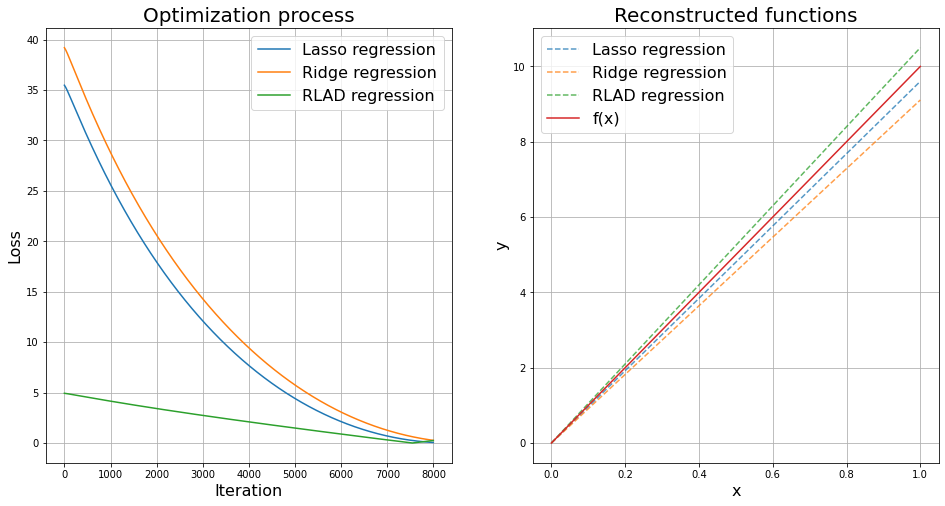
\includegraphics[width=\textwidth]{images/chapter2/reularization_impact.png}
	\caption{Comparison of different regularizations techniques}
	\label{fig:regularizations}
\end{figure}

\section{Regression as one of the types of expansion of function into functional series}
The linear regression model looks like expanding some unknown function in a series into predefined functions \eqref{eq:linear_expansion}. If we assume that $ \phi_i = cos $, then linear regression is transformed into an expansion of the function into a Fourier series, but without the mutual orthogonality of its terms. Instead of Fourier expansion, any functions, Chebyshev polynomials or Legendre polynomials can be used. In this section, we will discuss some expansions that are useful for further work.

\subsection{Fourier series}
Instead of arbitrary $\phi_i$ substitute $e^{i \pi k}$ to \eqref{eq:linear_expansion}:
\begin{equation*}
	\begin{multlined}
		S_K(x) = \beta_0 + \sum_{i = 1}^K \beta_i e^{i \pi k x} \implies S(x) = a_0 + \sum_{i = 1}^K \left (a_i cos(\pi k x) + b_i sin(\pi k x) \right ) \\
	\end{multlined}
\end{equation*}
This set of functions is orthogonal on the considered interval:
\begin{equation*} 
	\int_{-\pi}^{\pi} e^{i \pi k x} e^{i \pi l x} = 2\pi \delta_k^l 
\end{equation*}
The estimation of $a_n$ and $b_n$ for some function $f$ is a straightforward process, first of all, define the residual for this expansion - $R(x) = f(x) - S_K(x)$, after that, integrate the squared residual over the domain and use the least-squares method:
\begin{equation*}
	\begin{multlined}
		\mathcal{L} = \int_{\Omega} R(x)^2 d\Omega = \int_{\Omega} \left ( f(x) - S_K(x) \right )^2 d\Omega = \\ = \int_{\Omega} f(x)^2 d\Omega - 2 \int_{\Omega} S_K(x) f(x) d\Omega + \int_{\Omega} S_K(x)^2 d\Omega = \\ = \int_{\Omega} f(x)^2 d\Omega - 2 \int_{\Omega} \left [ a_0 + \sum_{i = 1}^K \left (a_i cos(\pi k x) + b_i sin(\pi k x) \right ) \right ] f(x) d\Omega + \\ +  \int_{\Omega} \left [ a_0 + \sum_{i = 1}^K \left (a_i cos(\pi k x) + b_i sin(\pi k x) \right ) \right ]^2 d\Omega
	\end{multlined}
\end{equation*}
And the derivates of the integrated residual:
\begin{equation}
 	\begin{multlined}
 		\begin{cases}
 			\dfrac{\partial }{\partial a_n} \mathcal{L} = \dfrac{\partial \mathcal{L}}{\partial S_K(x)} \dfrac{\partial S_K(x)}{\partial a_n}  = -2 {\displaystyle \int_{\Omega}} f(x) cos(\pi k x) d\Omega + -2 {\displaystyle \int_{\Omega}} S_K(x) cos(\pi k x) d\Omega \\[20pt]
 			\dfrac{\partial }{\partial b_n} \mathcal{L} = \dfrac{\partial \mathcal{L}}{\partial S_K(x)} \dfrac{\partial S_K(x)}{\partial b_n} = -2 {\displaystyle \int_{\Omega}} f(x) sin(\pi k x) d\Omega + -2 {\displaystyle \int_{\Omega}} S_K(x) sin(\pi k x) d\Omega \\[20pt]
 			\dfrac{\partial }{\partial a_0} \mathcal{L} = \dfrac{\partial \mathcal{L}}{\partial S_K(x)} \dfrac{\partial S_K(x)}{\partial a_0}  = -2 {\displaystyle \int_{\Omega}} f(x) d\Omega + 2 |\Omega| a_0 \\[20pt]
 		\end{cases}
 	\end{multlined}
 	% \mathcal{L} = \int_{\Omega} R(x)^2 d\Omega
\end{equation}
The main part of the calculations is absent and provided here \cite{fourierintro}. In addition, there is a convergence analysis of the coefficients, in sense of pointwise, and $L_2$ norm. The final result for the coefficients is:
\begin{equation}
	\begin{cases}
		a_0 = \dfrac{{\displaystyle \int_{\Omega}} f(x) d\Omega }{2 | \Omega |} \\[20pt]
		a_n = \dfrac{{\displaystyle \int_{\Omega}} f(x) cos(\pi k x) d\Omega}{| \Omega |} \\[20pt]
		b_n = \dfrac{{\displaystyle \int_{\Omega}} f(x) sin(\pi k x) d\Omega}{| \Omega |} \\[20pt]
	\end{cases}
\end{equation}

\paragraph{Example of function expansion into the Fourier series} 
Consider the function $y = sin(x) + x$ and at the fig. \ref{fig:fourier_demo} the results. It can be seen that with a relatively small amount of the terms the approximation good. With 3 terms the approximation error\footnote{Here, the approximation error is the loss function and concrete - mean squared error between the known values and Fourier expansion. There is a pointwise loss value, where the error calculation includes the finite number of nodes and integral loss value, where the residual integrates over the all domain.} is 0.565, 5 terms - 0.005 and 10 terms is 0.002.
\begin{figure}[h]
	\centering
	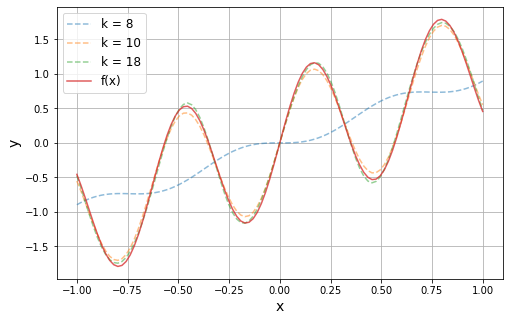
\includegraphics[width=\textwidth]{images/chapter2/fourier_demo.png}
	\caption{Example of function expansion into the Fourier series with 3, 10, 18 terms}
	\label{fig:fourier_demo}
\end{figure}

\subsubsection{The strong sides of Fourier expansion}
There are two important theorems helps to use Fourier expansion for construction of the future approximation:

\newtheorem{theorem}{Theorem}[chapter]
\begin{theorem}
\label{convergence-l2-norm}
If $f$ belongs to $L^{2}(\left[-\pi ,\pi \right])$ then $S_k$ converges to $f$ in $L^{2}(\left[-\pi ,\pi \right])$, that is, $\|S_K - f\|_{2}$ converges to 0 as $N \rightarrow \infty$.
\end{theorem}
\begin{theorem}
\label{convergence-pointwise}
If $f$ belongs to $C^1(\left[-\pi ,\pi \right])$ then $S_k$ converges to $f$ uniformly (and hence also pointwise).
\end{theorem}
The proofs of theorems well provided here \cite{fourierintro}. And an additional fact, Fourier coefficients of any integrable function tend to zero. 


\begin{figure}[h]
	\centering
	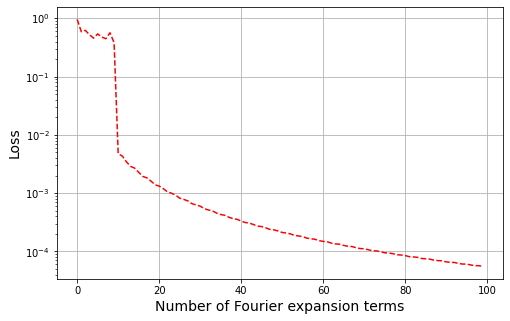
\includegraphics[width=\textwidth]{images/chapter2/fourier_quality.png}
	\caption{Illustration of the theorems \ref{convergence-l2-norm}, \ref{convergence-pointwise} for the function from the previous example}
	\label{fig:fourier_quality}
\end{figure}
\subsection{Chebyshev polynomials and Chebyshev series}
Again, instead of using trigonometric polynomials, you can apply another system of orthogonal polynomials - Chebyshev polynomials and expand the desired function in a Chebyshev series. A distinctive feature of the use of this system of polynomials is the fact that the Gibbs phenomenon is absent. The Gibbs phenomenon is a special case of the problem of the numerical representation of a function with sharp jumps through its Fourier series. Chebyshev polynomials can be defined as a recurrence sequence:
\begin{equation}
	T_0(x) = 1, T_1(x) = x, \dots, T_n(x) = 2 x T_{n - 1}(x) - T_{n - 2}(x)
\end{equation}
This polynomials are orthogonal with weight $w(x) = \dfrac{1}{\sqrt{1 - x^2}}, more details here$\cite{mason2002chebyshev}:
\begin{equation}
	\label{eq:chebyshev_series}
	\int_{-1}^{1} T_k(x) T_l(x) w(x) dx = \begin{cases}
		\pi \delta_l^k, k = 0, \\
		\cfrac{1}{2} \pi \delta_l^k, k \neq 0
	\end{cases}
\end{equation}
Examples of the first six polynomials are plotted at the \ref{fig:chebyshev_demo}
\begin{figure}[h]
	\centering
	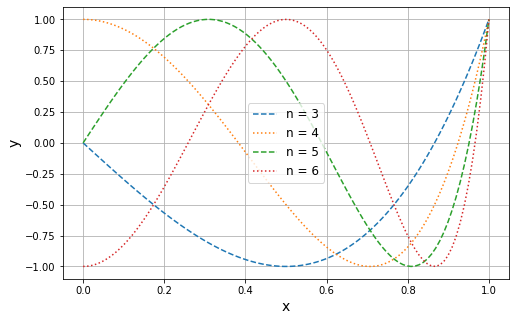
\includegraphics[width=\textwidth]{images/chapter2/chebyshev_demo.png}
	\caption{Chebyshev polynomias for n = 3, 4, 5, 6}
	\label{fig:chebyshev_demo}
\end{figure}

These polynomials are used for the interpolation procedure to avoid the Runge phenomenon\footnote{In the mathematical field of numerical analysis, Runge's phenomenon is a problem of oscillation at the edges of an interval that occurs when using polynomial interpolation with polynomials of high degree over a set of equispaced interpolation points.}, in case, when they are monic polynomials. Moreover, the roots of them often used in numerical linear algebra in method conjugated gradient descent, for example\footnote{
More information is here - ``E. Kaporin, Using Chebyshev polynomials and approximate inverse triangular
factorizations for preconditioning the conjugate gradient method, Zh. Vychisl. Mat.
Mat. Fiz., 2012, Volume 52, Number 2, 179–204``}.
The details of the Chebyshev polynomials is not important for this work, but there are a lot of benefit of using them in different problems.

Chebyshev series is the expansion of the function by his polynomials or, simply substitute polynomials to \eqref{eq:linear_expansion}:
\begin{equation*}
	\begin{multlined}
		f(x) = \sum_{k = 0}^{\infty} c_k T_k(x) \\
		c_k = \dfrac{1}{M} \int_{-1}^1 f(x) T_k(x) w(x) dx, \text{where } M = \begin{cases}
		\pi, k = 0, \\
		\dfrac{1}{2} \pi, k \neq 0
	\end{cases} \\
	\text{and } w(x) \text{ weight function } = \dfrac{1}{\sqrt{1 - x^2}}
	\end{multlined}
\end{equation*}
The convergence theorem of Chebyshev functional series:
\begin{theorem}
\label{chevyshev_convergence}
When a function $f$ has $m + 1$ continous derivatives on $[-1, 1]$ or $ f \in C^{m + 1}[-1, 1] $, where $m \in N^+$, then $\| f(x) - S_k(x) \| = \mathcal{O}\left ( \dfrac{1}{k^m} \right )$ as $k \rightarrow \infty \quad \forall x \in [-1, 1]$ 
\end{theorem}
The proof here \cite{mason2002chebyshev}.
This theorem described the same fact that theorem \ref{convergence-l2-norm}  described for the Fourier expansion.

For example, consider the function $y = sin(x) + x cos(x)$ and at the fig. \ref{fig:chebyshev_expansion} the results. 
\begin{figure}
	\centering
	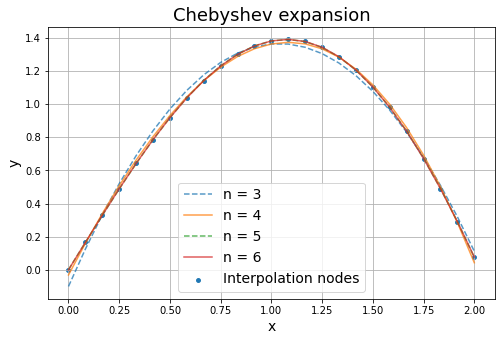
\includegraphics[width=\textwidth]{images/chapter2/chebyshev_series.png}
	\caption{Chebyshev expansion with 3, 4, 5, 6 terms }
	\label{fig:chebyshev_expansion}
\end{figure}
In fact, Chebyshev series is Generalized Fourier series: 
\begin{equation*}
	\begin{multlined}
		f(x) = \sum_{i = 1}^{N} c_n \phi_n(x) \\
		\left < \phi_i, \phi_j \right > = \int_{V} \phi_i \phi_j w dV = K_i^j
	\end{multlined}
\end{equation*}

\subsection{Another functions and expansion over them}
In case, when Generalized Fourier Series (GRS) is considered there are a lot of function can be used, for example\cite{abramowitz1965handbook}:
\begin{itemize}
	\item Gegenbauer polynomials
	\item Jacobi polynomials
	\item Romanovski polynomials
	\item Legendre polynomials
\end{itemize}

All have their own weight function and satisfy the GSR and potentially applicable for function approximation via the least-squares method and gradient-based methods with suitable penalty parameter (regularization term). In fact, during the approximation process (or supervised learning) includes fixation of the basis function, choice of the regularization. On the other hand, usage orthogonal functions for approximation or interpolation not restricted only GSR, actually, the linear regression model uses linearly-independent functions only.

\subsubsection{Function expansion over sigmoid function}
Let $\sigma = \dfrac{1}{1 + e^{-x}}$ and substitute to \eqref{eq:linear_expansion} instead of $\phi_i$ and apply an affine transformation to argument:
\begin{equation}
	\label{eq:sigmoidal_expansion}
	G(x) = \sum_{i = 1}^K \alpha_i \sigma(\beta_i x^j_i + \gamma_i)
\end{equation}
the expansion over the sigmoid functions is got. 
This expansion, in fact, one of the widely used in approximation process. First of all, there is a useful theorem that provides guarantees of the quality for approximation. 
\newpage
\begin{theorem}
	Let $\sigma = \dfrac{1}{1 + e^{-x}}$, then finite sums of the form:
	\begin{equation*}
		G(x) = \sum_{i = 1}^K \alpha_i \sigma(\beta_i x^j_i + \gamma_i)
	\end{equation*}
	are dense in $C(I_n\footnote{
	 Unit cube in $R^n$. The term unit cube or unit hypercube is also used for hypercubes, or "cubes" in $n$-dimensional spaces, for values of n other than 3 and edge length 1
	})$. In other words, given any $f \in C(I_n)\footnote{
		The space of continuous functions over $I_n$
	}, \epsilon > 0$, there is a sum, $G(x)$, of the above form, for which:
	 $\| G(x) - f(x) \| < \epsilon, \quad \forall x \in I_n$
\end{theorem}
In simple words, this theorem provides justification for the expansion of the function into the sigmoidal series, moreover, the quality of the approximation can be tremendously increased via increasing the terms in the series. By the way, the series \eqref{eq:sigmoidal_expansion} named neural network\footnote{Neural network, or Artificial neural networks (ANN) or connectionist systems are computing systems vaguely inspired by the biological neural networks that constitute animal brains. Such systems "learn" to perform tasks by considering examples, generally without being programmed with task-specific rules.} or perceptron\footnote{In machine learning, the perceptron is an algorithm for supervised learning of binary classifiers or regressor.} with one hidden layer and sigmoidal activation function. 

Coefficients for the expansion can be found via the least-squares method or using the gradient-based methods which more suitable when talking about neural networks. The question of estimating them is a future section question, but there is a lot of special algorithms for it.

\section{Differention equations}
\subsection{Introduction}
Differential equations can be split into two big groups:
\begin{itemize}
	\item Ordinary differential equations (ODE)
	\begin{itemize}
		\setlength\itemsep{0.5em}
		\item Single ODE
		\item System of ODEs
	\end{itemize}
	\item Partial differential equations (PDE)
	\begin{itemize}
		\setlength\itemsep{0.5em}
		\item Single PDE
		\item System of PDEs
	\end{itemize}
\end{itemize}
For each group, there are a lot of solving methods, for ODE (shooting method, Euler method, Runge–Kutta methods, and so on) or for PDE (Finite difference method, finite element method, finite volume method and so on). Most of them based upon the idea of numerical integration or function approximation via some sequence of function and the minimization of the residual, for example, weighted residuals method \cite{finlayson2013method} \cite{fletcher2012computational}. All of these methods lead to solving the system of algebraic equations, in the general case. In case when the equation is simple enough the system of linear equations should be solved. Suppose that after applying some numerical method for some problem and not important for what method and what problem, a linear system is got: 
% \kappa (A) = \| A \| \| A^{-1} \|$ - condition number
$A x = b$, let $b = \hat{b} + e_b $, where $e_b$ is error in vector $b$ it can be caused by rounding errors or predefined errors related to data collection if speech going about real problems of the oil and gas industry, for example. Here the existence of this error is interesting because the solution error implies from the error in the left-hand side and can be larger than her. $x = A^{-1} (\hat{b} + e) = A^{-1} \hat{b} + A^{-1} e_b$, and $x = \hat{x} + e_x = A^{-1} \hat{b} + A^{-1} e_b$ and:
\begin{equation*}
	\begin{cases}
		\hat{x} = A^{-1} \hat{b} \\
		e_x = A^{-1} e_b
	\end{cases} \implies \max_{e, b} \dfrac{\|A^{-1} e_b\|}{\|A^{-1} \hat{b} \|} \dfrac{\|b\|}{\|e_b\|} = \| A \| \| A^{-1} \| = \kappa(A)
\end{equation*}
$\kappa(A)$ - condition number\cite{gentle2007matrix}. 

It means that if the matrix has a large value of the condition number then the error of the $x$ is large\footnote{The influence of the condition number on the solution accuracy presented at the fig. \ref{fig:ill_condition_demo}. Here considered the model example of the linear system, with $\kappa = 3422.83$ and presented the components of the vector b and his deviations, then x was found and deviations. It can be seen that the deviations of b (left part, blue circles) near the initial values(red line), but the deviations for x has a large spreading. This is an influence of condition number.}.
This fact leads to the use of preconditioners to decrease the condition number and gets a more stable solution. There are a lot of ways to preconditioning the system of linear equations: Jacobi (or diagonal) preconditioner, incomplete Cholesky factorization, incomplete LU factorization, and so on. 

It is one of the problems that arise during the ODE/PDE solving but in fact, there are problems such as convergence rate, mesh generation, interpolation of the solution, choose the function for approximation, and so on. In this work don't provide the method that ideal and works well for all problems, but for the presented in the continuation, problems work fast and well. In fact, if the method won't depend on the mesh and use only the randomly chosen points and will work well for some problems - it will be a small victory. 

\begin{figure}[h]
	\centering
	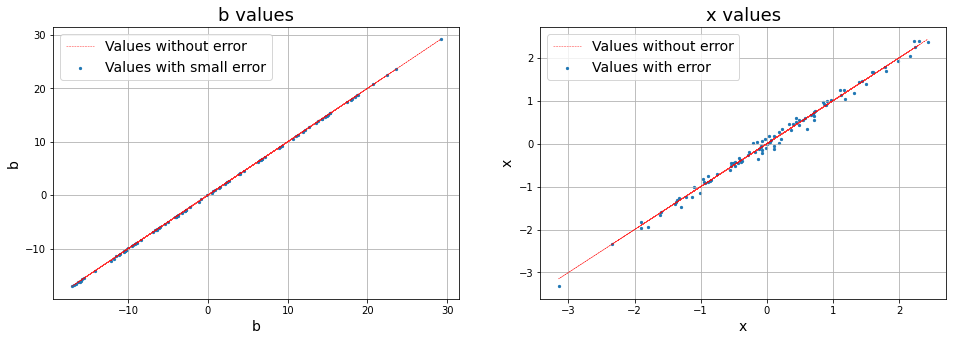
\includegraphics[width=1.0 \textwidth]{images/chapter2/ill_condition_demo.png}
	\caption{The influence of the condition number on the solution accuracy}
	\label{fig:ill_condition_demo}
\end{figure}
\subsection{The solution of differential equations (DE)}
In this section, we will consider some arbitrary ordinary differential equation of order $n$ and the corresponding boundary conditions::
\begin{equation}
	\label{eq:ode}
	\begin{multlined}
		\mathcal{D}\left (x, y, y^{(1)}, \dots, y^{(n)}\right) = 0, \quad x \in \Omega = [0, 1] \subset  R \\
		B(y) = 0, \quad x \in \partial \Omega = \{0, 1\}
	\end{multlined}
\end{equation}
, where $\mathcal{D}(\dots)$ - arbitrary smooth nonlinear function, $B(y)$ - function characterizing the boundary conditions. 
\begin{equation*}
	B(y) = \begin{cases}
		D(y) = 0, \quad x \in \partial \Omega_D = \{0, 1\} \\
		N(y) = 0, \quad x \in \partial \Omega_N = \{0, 1\} 
	\end{cases}, \partial \Omega_N \cup \partial \Omega_D = \partial \Omega
\end{equation*}
бwhere $D(y)$ - Dirichlet boundary conditions and $\partial \Omega_D$ boundary for these conditions, N(y) - Neumann boundary conditions and $\partial \Omega_N$ is bound them.
All of the equations considered now and in the future in this work will be defined as \eqref{eq:ode}.
For solving this equation will be considered two methods, weighted residuals method \cite{fletcher2012computational} (Bubnov-Galerkin) and finite differences method \cite{dimov2019finite}.

\subsubsection{Galerkin method}
The key idea is to define the solution as:
\begin{equation}
	\label{eq:galerkin_presentation}
	y_h = \phi_0 + \sum_{i = 1}^N a_i \phi_i(x)
\end{equation}
and $\phi_0$ satisfy all boundary conditions $\phi_0: B(\phi_0) = 0 \implies \phi_0(0) = 0, \phi_0(1) = 1$ and $\phi_i$ satisfy the homogenous boundary conditions $\phi_i(0) = \phi_i(1) = 0$. The solution to the problem is a some weighted sum of linearly independent functions that satisfy the boundary conditions and in the general case satisfy the initial conditions too. For calculation, the coefficients use minimization residual method, where:
\begin{equation*}
	\min_{a_1, \dots, a_n} R(a_1, \dots, a_n) = \int_{\Omega} \mathcal{D}(y_h) d\Omega + \int_{\partial \Omega_N} N(y_h) d\partial \Omega
\end{equation*}
From \cite{fletcher2012computational} is known that $R$ does not equal zero in the general case and for evaluating the coefficients use the integration with weight function:
\begin{equation*}
	\int_{\Omega} w R(a_1, \dots, a_n) d\Omega = \int_{\Omega} w \mathcal{D}(y_h) d\Omega + \int_{\partial \Omega_N} w N(y_h) d\partial \Omega = 0
\end{equation*}
, where $w = \psi_i$, weight functions. The residual and weight functions must be orthogonal.
In a more general case without using $phi_0$ the residual is:
\begin{equation*} 
	\begin{multlined}
		\int_{\Omega} \psi_j R(a_1, \dots, a_n) d\Omega = \int_{\Omega} \psi_i \mathcal{D} \left ( \sum_{i = 1}^N a_i \phi_i(x) \right ) d\Omega + \int_{\partial \Omega} \psi_j B \left ( \sum_{i = 1}^N a_i \phi_i(x) \right ) d\partial \Omega = \\ =
		\int_{\Omega} \psi_j \mathcal{D} \left ( \sum_{i = 1}^N a_i \phi_i(x) \right ) d\Omega + \int_{\partial \Omega} \psi_j B \left ( \sum_{i = 1}^N a_i \phi_i(x) \right ) d\partial \Omega = \text{ if $\mathcal{D}, \mathcal{B}$ are linear operators } = \\ = \int_{\Omega} \sum_{i = 1}^N  a_i \psi_j \mathcal{D}(\phi_i(x)) d\Omega + \int_{\partial \Omega} \sum_{i = 1}^N  a_i \psi_j B(\phi_i(x)) d\partial \Omega = 0
	\end{multlined}
\end{equation*}
From the equation above system of algebraic equations can be constructed and solve it for unknown coefficients $a_i$.
\subsubsection{Galerkin method, special case}
If $w$ is delta Dirac function, then the Galerkin method also called the Pointwise collocation method, which more easy for implementation.
\begin{equation}
	\begin{multlined}
		w = \delta(x - x_k), x_k \in X \subset \Omega, \text{ and } \| X \| = K, \\
		\int_{\Omega} \delta(x - x_k) R(a_1, \dots, a_n) d\Omega = \int_{\Omega} \delta(x - x_k) \mathcal{D} \left ( \sum_{i = 1}^N a_i \phi_i(x) \right ) d\Omega + \\ + \int_{\partial \Omega} \delta(x - x_k) B \left ( \sum_{i = 1}^N a_i \phi_i(x) \right ) d\partial \Omega
		 = \mathcal{D} \left ( \sum_{i = 1}^N a_i \phi_i(x_k) \right ) + B \left (\sum_{i = 1}^N a_i \phi_i(x_k) \right )
	\end{multlined}
\end{equation}
In case when the number of points of collocation more then the number of unknown coefficients the problem solves via optimization techniques, the least-squares method for example.

\subsubsection{Finite difference method}
First of all, the finite difference derivative is:
\begin{itemize}
	\item Left derivative \begin{equation}
		\label{eq:left_der}
		\dfrac{d y}{d x} \Big|_{x = x_i} = \dfrac{y(x_i) - y(x_{i - 1})}{x_i - x_{i - 1}}
	\end{equation}
	\item Central derivative \begin{equation}
		\label{eq:central_der}
		\dfrac{d y}{d x} \Big|_{x = x_i} = \dfrac{y(x_{i + 1}) - y(x_{i - 1})}{x_{i + 1} - x_{i - 1}}
	\end{equation}
	\item Right derivative \begin{equation}
		\label{eq:right_der}
		\dfrac{d y}{d x} \Big|_{x = x_i} = \dfrac{y(x_{i + 1}) - y(x_i)}{x_{i + 1} - x_i}
	\end{equation}
\end{itemize}
Actually, the approximation quality better for the central difference derivative. The derivatives of higher order can be constructed from the first-order derivatives (left, right, central). For example:
\begin{equation*}
	\dfrac{d^2 y}{d x^2} \Big|_{x = x_i} = \dfrac{d}{d x} \Big|_{x = x_i} \left [ \dfrac{y(x_{i + 1})}{x_{i + 1} - x_i} \right ] - \dfrac{d}{d x} \Big|_{x = x_i} \left [ \dfrac{y(x_{i - 1})}{x_i - x_{i - 1}} \right ] = \dfrac{y(x_{i + 1}) - y(x_i)}{x_{i + 1} - x_i} - \dfrac{y(x_i) - y(x_{i - 1})}{x_i - x_{i - 1}}
\end{equation*}
When the grid uniformly distributes the $x_i$ values: $x_{i + 1} - x_i = d$:
\begin{equation*}
	\dfrac{d^2 y}{d x^2} \Big|_{x = x_i} = \dfrac{y(x_{i + 1}) - 2 y(x_i) + y(x_{i - 1})}{d^2}
\end{equation*}
So, the idea of the FDM is to substitute the finite derivatives and solve algebraic equations. 
\begin{equation*}
	\mathcal{D} (x, y, y^{(1)}, \dots, y^{(n)}) \Big|_{x = x_i} = \mathcal{D} \left ( x_i, y(x_i), \dfrac{y(x_{i + 1}) - y(x_{i - 1})}{x_{i + 1} - x_{i - 1}}, \dots, \dfrac{y(x_{i + n - 1}) + \dots + y(x_{i - n + 1})}{d^n} \right )
\end{equation*}
And the same way for the boundary conditions:
\begin{equation*}
	B(y) \Big|_{x = x_i}  = \begin{cases}
		D(y) = 0, \quad x \in \partial \Omega_D = \{0, 1\} \\
		N(y) = 0, \quad x \in \partial \Omega_N = \{0, 1\} 
	\end{cases} 
\end{equation*}
After the solving equations, the values of $y_i$ are known and needed to be interpolated over the domain $\Omega$.
\subsubsection{Comparison of the provided methods}	
Methods are very different, the FDM provides the solution in the fixed nodes and interpolates the solution from these nodes overall domain, on the other hand, the Galerkin method provides approximation solution in the mean sense over the domain. This difference makes the variability of the interpolation methods or basis functions for calibration of the numerical solution quality. The strong and ill sides of the FDM are high quality of the solution over the nodes, but the interpolation process leads to the Runge phenomenon, besides the size of the grid has a tremendous influence on the solution quality. 
The Galerkin method provides the approximation over the domain and strongly depends on the initial choice basis functions, so, there is the probability, that solution has a compact form.

It will be good if the strong sides of these methods will be combined into one approximator. Ideal case, when the number of terms increases, the solution quality increase too.

First of all, using the theorem \ref{sigmoidal_expansion} and the solution form \eqref{eq:galerkin_presentation}:
\begin{equation}
	\label{eq:perceptron_ode}
	y_h(x) = \phi_0(x) + \sum_{i = 1}^K \alpha_i \sigma(\beta_i x + \gamma_i)
\end{equation}
$\phi_0$ also satisfy the boundary conditions. 
For this solution from the theorem known, that the approximation quality strongly depends on the number of terms in the series, in addition, this form satisfies the boundary conditions, as in the Galerkin method. Now, the quality of the solution is guaranteed by the theorem and the question about basis function is solved. Moreover, using points collocation method:
\begin{equation}
	\label{eq:loss_galrekin}
	\begin{multlined}
		\mathcal{L} = \dfrac{1}{| X |} \sum_{x \in X} \left [ \| R(x; p_1, 
		\dots, p_N) \|^2 \right ], \quad X \in \Omega \subset R, p_i = (\alpha_i, \beta_i, \gamma_i) \in P \subset R^3 \\
		\textbf{Coefficients :} \min_{p_i} \mathcal{L} = \begin{cases}
			\dfrac{\partial \mathcal{L}}{\partial \alpha_i} = 0 \\[10pt]
			\dfrac{\partial \mathcal{L}}{\partial \beta_i} = 0 \\[10pt]
			\dfrac{\partial \mathcal{L}}{\partial \gamma_i} = 0
		\end{cases}
	\end{multlined}
\end{equation}
Currently, the solution is found using the least-squares method, which leads to solving the system of equations with not one solution. For each solution, the loss function should be calculated and chose the parameter where problem has a minimum value.

For this approach calculation of the derivatives for a differential operator should be provided:
\begin{equation}
	\label{eq:bad_system}
	\begin{multlined}
		\dfrac{d y_h}{d x} = \dfrac{d}{d x} \left [ \phi_0(x) + \sum_{i = 1}^K \alpha_i \sigma(\beta_i x + \gamma_i) \right ] = \dfrac{d}{d x} \phi_0(x) + \sum_{i = 1}^K \alpha_i \dfrac{d}{d x} \sigma(\beta_i x + \gamma_i) = \\ = \dfrac{d}{d x} \phi_0(x) + \sum_{i = 1}^K \alpha_i \beta_i  \sigma(\beta_i x + \gamma_i) (1 - \sigma(\beta_i x + \gamma_i))
	\end{multlined}
\end{equation}
The form of the derivative immediately told that the solving of equations \eqref{eq:bad_system} is very unstable and there are a lot of roots. On the other hand, using the numerical derivative \eqref{eq:left_der}, \eqref{eq:central_der}, \eqref{eq:right_der} leads to:
\begin{equation}
	\label{eq:good_system}
	\begin{multlined}
		\dfrac{d y_h}{d x} \Big|_{x = x_i} \approx \dfrac{y_h(x_{i + 1}) - y_h(x_{i - 1})}{2d} = \dfrac{1}{2d} \left [ y_h(x_{i + 1}) - y_h(x_{i - 1}) \right ]
	\end{multlined}
\end{equation}

\subsubsection{Artificial neural networks (ANN)}	
Definition from Wikipedia is ``Artificial neural networks (ANN) or connectionist systems are computing systems vaguely inspired by the biological neural networks that constitute animal brains. Such systems "learn" to perform tasks by considering examples, generally without being programmed with task-specific rules``, or the second one definition: ``A mathematical model, as well as its software or hardware implementation, built on the principle of organization and functioning of biological neural networks - networks of nerve cells of a living organism.''

\begin{figure}[h]
	\centering
	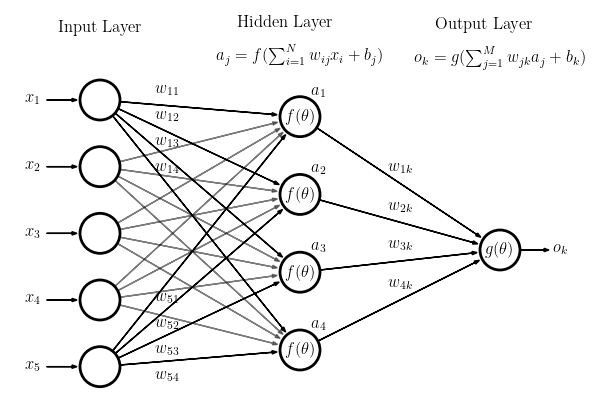
\includegraphics[width=\textwidth]{images/chapter2/neural_network_fcn.png}
	\caption{The illustration of \eqref{eq:perceptron_ode}. One layered neural network}
	\label{fig:simple_net}
\end{figure}

\begin{figure}[h]
	\centering
	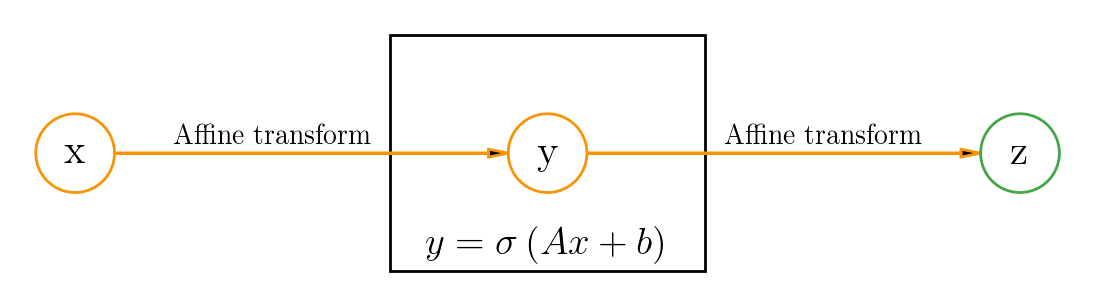
\includegraphics[width=\textwidth]{images/chapter2/simple_net.png}
	\caption{The illustration of \eqref{eq:perceptron_ode}. One layered neural network}
	\label{fig:simple_net}
\end{figure}

These definitions are similar, in the sense that the input signal passes through the set of ordered simple operations or layers, and at the end of these operations the output is the result of the neural network. The order of these operations also called the architecture of the neural network. There are a lot of different types of layers\footnote{The zoo of neural network types: \href{https://www.asimovinstitute.org/neural-network-zoo/}{ANN zoo}}, the most widely used is the fully connected layer or dense layer as in figure \ref{fig:simple_net}.
Looking more precisely the neural network is sequence of affine transformations (edges) and nonlinear transformation (nodes):
\begin{equation*}
	\begin{multlined}
		\mathcal{N}(x) = \left [ A^2 \circ \phi^1 \circ A^1 \right ] (x) = A^2 \phi^1 \left (A^1 x + b^1 \right ) + b^2 \\ A^1 \in R^{m \times n}, A^2 \in R^{k \times m}, b^1 \in R^m, b^2 \in R^k, x \in R^n
	\end{multlined}
\end{equation*}
In general case $l$ layered neural network is:
\begin{equation}
	\label{eq:neural_net}
	\mathcal{N} = A^l \circ \phi^{l - 1} \circ A^{l - 1} \circ \dots \circ \phi^1 \circ A^1 = A^l \left [ \phi^{l - 1} \left [ \dots \left [ A^1 (x) + b^1 \right ] \dots \right ] + b^{l - 1} \right] + b^l
\end{equation}
where $A^i, \forall i \in \{1, \dots, l\}$ is the parameter that must be found. For the successful using the neural networks:
\begin{itemize}
	\item Define the architecture
	\item Define the loss function
	\item Choose a suitable optimization algorithm \begin{itemize}
		\item How the optimization process looks
		\item Existing optimization algorithms
	\end{itemize}
\end{itemize}

\subsubsection{Optimization part. Backpropagation algorithm}

The main goal is getting the numerical solution of the DE and for this aim is to use the residual \eqref{eq:loss_galrekin} and minimize it over the parameters of the neural network:
\begin{equation*}
	\min_{A^l, b^l, \dots, A^1, b^1} \mathcal{L} = \min_{A^l, b^l, \dots, A^1, b^1} \mathcal{L} = \dfrac{1}{| X |} \sum_{x \in X} \| R(x) \|^2
\end{equation*}
Now, how to minimize this complex function? Using the least-squares leads to solving the equations or use gradient-based optimization. For the estimation, the values of the neural network parameters use the gradient-based methods and iteratively goes to the local minimum(!). Suppose, the for the point collocation method randomly choose the set of points at the $k$-th step, the loss is calculated and gradients are calculated:.
\begin{equation}
	\nabla A_k^l = \nabla_{A^l} \mathcal{L}_k, \quad A_{k + 1}^l = A_k^l - \lambda(k) \psi(\nabla A_k^l)
\end{equation}
the $\psi$ is the main part of the particular algorithm because using the $\psi(x) = x$, stochastic gradient descent (SGD) immediately have gotten. Using different $\psi$, the corresponding methods are obtained \cite{Adadelta}, \cite{Adagrad}, \cite{Adam}, \cite{Diffgrad}.
\paragraph{Optimizers comparison}
To demonstrate the quality of various optimization algorithms, a simple neural network architecture was chosen and trained to approximate the function. Lines are the average value of the loss function at a particular iteration, the region of the corresponding color is the region in which the error may lie on average. To collect such statistics, the neural network was trained by each optimizer 25 times.
The results are presented in the figure \ref{fig:optimizers}.
\begin{figure}[h]
	\centering
	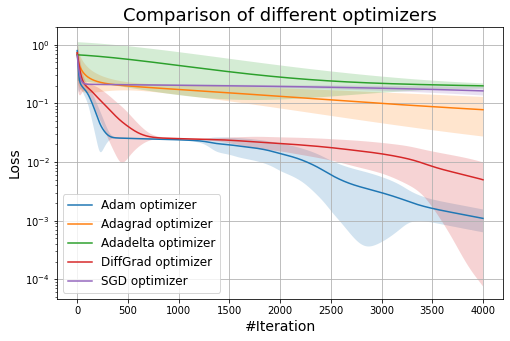
\includegraphics[width=\textwidth]{images/chapter2/optimizers.png}
	\caption{Comparison of different optimizers for fixed neural network architecture}
	\label{fig:optimizers}
\end{figure}


Consider the sequence of the operators \eqref{eq:neural_net} and the quality function or loss function $\mathcal{L}$. Currently not important what loss function and the nature of the operators:
\begin{equation*}
	\begin{multlined}
		\mathcal{N} = A^l \circ \phi^{l - 1} \circ A^{l - 1} \circ \dots \circ \phi^1 \circ A^1, \quad \mathcal{L} = \mathcal{L} \left ( \mathcal{N} \right )
	\end{multlined}
\end{equation*}
For efficient evaluating the gradients over the parameters exists a backpropagation\footnote{
	In machine learning, backpropagation (backprop, BP) is a widely used algorithm in training feedforward neural networks for supervised learning. Generalizations of backpropagation exist for other artificial neural networks (ANNs), and for functions generally – a class of algorithms referred to generically as "backpropagation" - from Wikipedia
} algorithm \cite{chauvin2013backpropagation}. The key idea is to use the chain rule for the derivative:
\begin{equation*}
	\begin{cases}
		\dfrac{\partial \mathcal{L}}{\partial A^l} = \nabla_{A^l}\mathcal{L} \\[10pt]
		\dfrac{\partial \mathcal{L}}{\partial A^{l - 1}} = \left [ \phi^l \right ]^{'} \left [ A^{l - 1} \right ]^T \nabla_{A^l}\mathcal{L} \\[10pt]
		\dfrac{\partial \mathcal{L}}{\partial A^{l - 2}} = \left [ \phi^{l - 1} \right ]^{'} \left [ A^{l - 2} \right ]^T  \left [ \phi^l \right ]^{'} \left [ A^{l - 1} \right ]^T \nabla_{A^l}\mathcal{L} =  \left [ \phi^{l - 1} \right ]^{'} \left [ A^{l - 2} \right ]^T  \dfrac{\partial \mathcal{L}}{\partial A^{l - 1}} \\[10pt] 
		\text{For k-th derivative in the same way:} \\[10pt]
		\dfrac{\partial \mathcal{L}}{\partial A^{l - k}} = \left [ \phi^{l - k + 1} \right ]^{'} \left [ A^{l - k} \right ]^T  \dfrac{\partial \mathcal{L}}{\partial A^{l - k + 1}}
	\end{cases} 
\end{equation*}
Now it is known how a neural network works, how it is trained and why a solution can be built with arbitrary accuracy. Next, we will consider different architectures of neural networks for solving different problems, and different approaches, for example, the approach based on the Galerkin method, when the Dirichlet boundary conditions are embedded in a neural network. There is also an approach based on the Ritz method that reduces the solution of the equation to an extremal problem. For example, when solving equations, it is possible to integrate the boundary conditions into the approximator structure \cite{Lagaris_1998} \cite{liu2019solving}.
Here the solution is presented in the form:
\begin{equation}
	\label{eq:simple_solver}
	y_h = A(x) + B(x) \mathcal{N}(x)
\end{equation}
where $A$ satisfies the boundary conditions of the first and second kind, where $A$ satisfies the boundary conditions of the first and second kind, and $B$ is in a sense a function of distance, or rather a function that “removes” the values of the model (neural network) at the boundary. 

Consider equation $\phi \left ( x, y, \dfrac{d y}{d x}, \dfrac{d^2 y}{d x^2} \right ) = 0$ and boundary conditions $y(0) = y_0, y(1) = y_1$. In this case, the solution will be built in the form:
\begin{equation*}
	y_h = (1 - x) y_0 + x y_1 + (1 - x) x \mathcal{N}(x)
\end{equation*}
Thus, for such a form, a neural network is only part of the solution, for points within a region. It is clear that the name of the complex boundary conditions for the partial differential equation to construct a solution in this form is very difficult. In this form, it is convenient to search for a solution having homogeneous boundary conditions of the first kind. You can use the results from \cite{fletcher2012computational}, where it is proposed to construct the solution in such a way as to satisfy only conditions of the first kind, and transfer conditions of the second and third kind to the neural network again (to the loss function), example:
\begin{equation*}
	\begin{multlined}
		\phi \left ( x, y, \dfrac{d y}{d x}, \dfrac{d^2 y}{d x^2} \right ) = 0, \quad y(0) =  y_0, \dfrac{d y}{d x} \Big|_{x = 0} = y_1 \\
		y_h = (1 - x) y_0 + B(x) \mathcal{N}(x), \quad \mathcal{L}^{'} = \mathcal{L} + \lambda \left \| \dfrac{d y_h}{d x}\Big|_{x = 0} - y_1  \right \|
	\end{multlined}
\end{equation*}
Another approach \cite{cao2016locally} also embeds the boundary conditions in the general solution, however, it occurs due to an additional term that estimates the error between the conditions and the solution itself at the boundary and embeds the additional term in a row in order to satisfy the conditions. In fact, every few iterations of the network training, the term is recalculated (a small system of equations is solved) and adjusted to the boundary conditions. Not quite an easy way to implement, however, the quality of the final solution depends on the boundary conditions, on the structure of the additional unit and the necessary accuracy. Models based on the Galerkin method are quite common, so the authors \cite{Sirignano_2018} proposed the structure of the model so that, with an increase in the dimension of the problem, the quality of the solution remains acceptable. Their model looks interesting, combines many breakthrough deep learning approaches, but in view of this, the speed of learning is very low. The authors themselves in their work provide an assessment of the training time and the necessary capacities for this - it takes an order of magnitude more time on a conventional personal computer than classical approaches require, but the main goal is high-dimensional tasks, where the algorithm really showed good quality. All approaches proposed and considered below can be divided into 2 groups: 
\begin{itemize}
	\item Embed in the solution itself \cite{Lagaris_1998} \cite{liu2019solving} \cite{cao2016locally}
	\item Consider a conditional problem solved by the Lagrange method. In the learning process, the model learns not only to solve the equation itself, but is also fined for not satisfying the boundary conditions \cite{Pun_2019}
\end{itemize}
Each group has its own characteristics, so for methods from the first group, the high quality of the solution is characteristic, but the difficulty of drawing up the presentation of the solution is high. The second group is characterized by a not very high quality solution, especially at the borders, however, with sufficient training time and properly selected regularization, this problem is solved, but the plus is the ease of implementation.

For the demonstration of the proposed approach consider the first example - ODE:
\begin{equation*}
	\dfrac{d y}{d x} = sin(x), \quad y(0) = -1
\end{equation*}

The loss function for the training neural network:
\begin{equation}
	\begin{multlined}
		\mathcal{N} = A^1 \sigma \left [ A^0 x + b^0 \right ] + b^1 \\
		\mathcal{L} = \sum_{x_k \in X} \left [ \dfrac{d}{d x} \mathcal{N} \big|_{x = x_k} - sin(x_k) \right ]^2 + \lambda \left [  \mathcal{N} \left( 0 \right ) + 1 \right ]^2 \\
		\left ( \hat{A}^1, \hat{A}^0, \hat{b}^1, \hat{b}^0 \right ) = \min_{A^1, A^0, b^1, b^0} \mathcal{L} = \min_{A^1, A^0, b^1, b^0} \sum_{x_k \in X} \left [ \dfrac{d}{d x} \mathcal{N} \big|_{x = x_k} - sin(x_k) \right ]^2 + \\ + \lambda \left [  \mathcal{N} \left( 0 \right ) + 1 \right ]^2
	\end{multlined}
\end{equation}

\begin{table}
	\centering
	\begin{tabular}{| c | c | c |} 
	\hline
		Method & Parameters num & Accuracy \\
		\hline FDM & 10  & $7.82 10^{-3}$  \\ 
		FDM & 25  & $2.88 10^{-3}$  \\
		FDM & 50  & $1.44 10^{-3}$  \\
		FDM & 100  & $0.69 10^{-3}$ \\
		FDM & 200  & $0.34 10^{-3}$ \\
		ANN & 8  & $0.298 10^{-3}$  \\
		ANN & 10  & $0.111 10^{-3}$ \\
		ANN & 20  & $0.0105 10^{-3}$  \\
		ANN & 50  & $0.00413 10^{-3}$ \\ \hline
	\end{tabular}
	\caption{Accuracy of the solution for different number of the parameters}
	\label{table:ode1_tab}
\end{table}

\begin{figure}
	\centering
	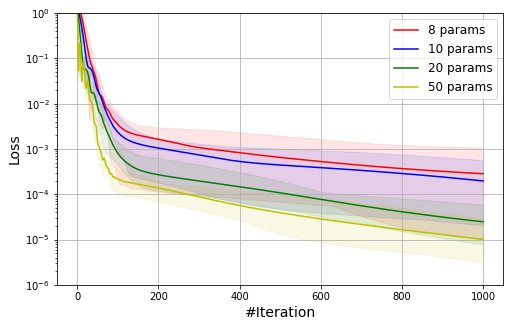
\includegraphics[width=\textwidth]{images/chapter2/ode1-training-info.png}
	\caption{Training process for several}
	\label{fig:ode1}
\end{figure}

\begin{figure}
	\centering
	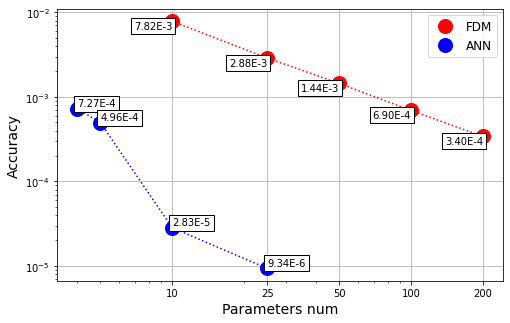
\includegraphics[width=\textwidth]{images/chapter2/fdm_ann_ode_1.png}
	\caption{Graphical description of the table \ref{table:ode1_tab}}
	\label{fig:fdm_ann_ode1}
\end{figure}

The training process on the figure \ref{fig:ode1} describes the solving process and the values of the loss per training iteration for $n$ independent launches. So, it is important, because in fact, when the neural network created, parameters initialized randomly using algorithms presented by \cite{glorot2010understanding} \cite{he2015delving} \cite{saxe2013exact}. 
The comparison of the FDM solution and the neural network solution describes table \ref{table:ode1_tab}. In this work was used Xavier initialization for all networks. For the convenience of the analysis the table \ref{table:ode1_tab} results presented in figure \ref{fig:fdm_ann_ode1}. Here it can be seen that the accuracy of the FDM increases linearly on the logarithm-logarithm plot, which means, that for the decrease the loss function on the 1 order is possible if the number of the parameters will increase in 2 times.

Future analysis will be provided in some steps, first is to apply a neural network-based solver to some number of the ODE's, simple linear, nonlinear, and for the system. The next step includes the application of the solver to single PDE, like the Poisson equation and wave equation, one nonlinear ODE. The last step will be provided for the system's of the PDEs: Stokes equation and Linear elasticity equations. Each of the presented steps will include the comparison of the used number of the parameters for the ANN and for the numerical method, such as FDM or FEM.

\subsection{The solution of systems of ordinary differential equations (S-ODE)}
The solution of a system of ordinary differential equations reduces to the solution of each equation separately, with other functions already known. The idea is to replace each function with a neural network, or use one with several outputs, where each output is a separate function. The loss function will be the sum of the loss function for each equation in the system.

As an example, the system of equations \eqref{eq:ode_sys_1}  will be solved.
\begin{equation}
	 \label{eq:ode_sys_1}
	\begin{cases}
		\dfrac{d x}{d t} = sin(t) - y \\[10pt]
		\dfrac{d y}{d t} = cos(t) + x \\[10pt]
		x(0) = x_0, y(0) = y_0
	\end{cases}
\end{equation}

To apply the proposed approach, it is necessary to formulate the objective function:
\begin{equation}
	\label{eq:loss_ode_sys_1}
	\begin{multlined}
		\mathcal{N} = [ \mathcal{N}_x, \mathcal{N}_y ]^T, \quad
		\begin{cases}
			\dfrac{d x}{d t} = sin(t) - y \\[10pt]
			\dfrac{d y}{d t} = cos(t) + x \\[10pt]
			x(0) = x_0, y(0) = y_0
		\end{cases} \implies \mathcal{L} = \mathcal{L}_1 + \mathcal{L}_2 + \mathcal{L}_{\text{boundary}} \\ \mathcal{L} = \dfrac{1}{\left | T \right |} \sum_{t \in T \subset R} \left [ \dfrac{d \mathcal{N}_x}{d t} - sin(t) + \mathcal{N}_y \right ]^2 + \\ + \dfrac{1}{\left | T \right |} \sum_{t \in T \subset R} \left [ \dfrac{d \mathcal{N}_y}{d t} - cos(t) - \mathcal{N}_x \right ]^2 + \\ + \lambda_1 \left [ \mathcal{N}_x \right ]^2 \big|_{t = 0} + \lambda_2 \left [ \mathcal{N}_y \right ]^2 \big|_{t = 0}
	\end{multlined}
\end{equation}

\begin{figure}
	\centering
	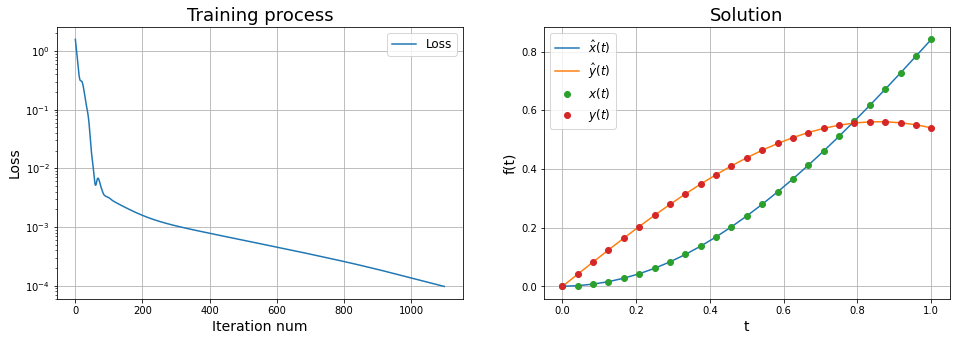
\includegraphics[width=1 \textwidth]{images/chapter2/ode_sys_1_res.png}
	\caption{Solution of equation \eqref{eq:ode_sys_1}, $\quad \mathcal{L} = 2.14565 \cdot 10^{-7} $ }
	\label{fig:ode_sys_1_res}
\end{figure}

Figure \ref{fig:ode_sys_1_res} the left part is the process of minimizing the error function, the right part is the result of a solution using a neural network - lines and the analytical solution - circles. It can be seen that the solution coincides, despite the fact that only 18 parameters are used in the neural network.

\subsection{The solution of partial differential equations (PDE)}

To solve partial differential equations, the same approach is used as for solving ordinary differential equations. By example, the Poisson equation will be solved.

\begin{equation*}
	\nabla^2 u = f(x), \quad \nabla^2 = \nabla \cdot \nabla, \forall x \in \Omega
\end{equation*}

\begin{table}
	\centering
	\begin{tabular}{| c | c | c |} 
		\hline
		$f(x) = $ & Solution & Equation number \\ \hline
		$ -2 sin(x) cos(y) $ & $ y = sin(x) cos(y) $ & 1\\
		$ 2 y^2 + 2 x^2 $ & $ y = x^2 y^2 $ & 2\\ \hline
	\end{tabular}
	\caption{Examples of equations to consider}
	\label{table:pde1_tab}
\end{table}

The results of solving each equation are presented in graphs \ref{fig:pde_1_1}, \ref{fig:pde_1_2}. To solve the equations, we considered a network structure including 1 one with a sigmoidal activation function. The process of training a neural network took about 10 seconds, which is quite a long time, but it is important to understand that the number of parameters is 18, which is very small for construction and the convergence to the solution is slow because of this.

\begin{figure}
	\centering
	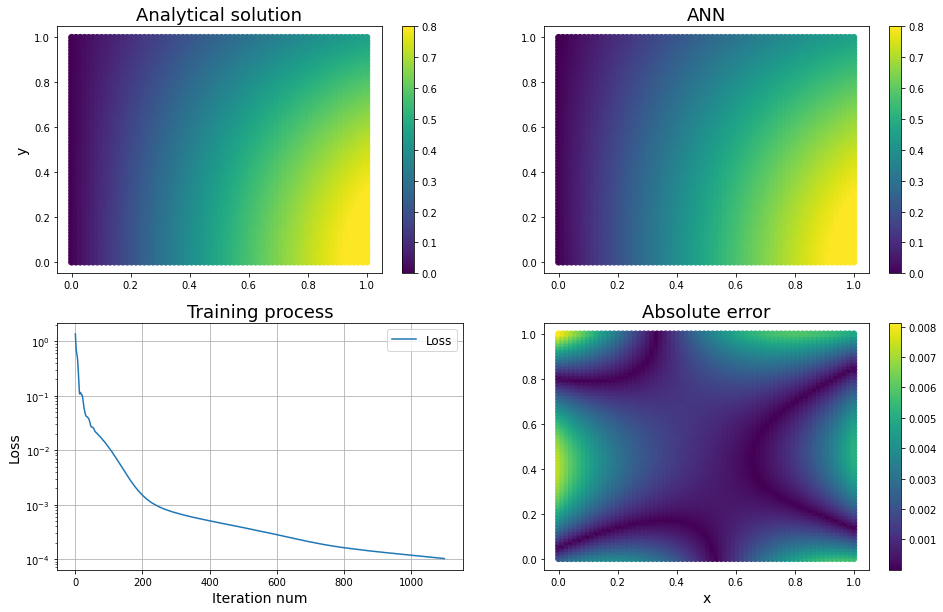
\includegraphics[width=\textwidth]{images/chapter2/pde_1_1.png}
	\caption{Solution of equation 1 from the table \ref{table:pde1_tab}}
	\label{fig:pde_1_1}
\end{figure}

\begin{figure}
	\centering
	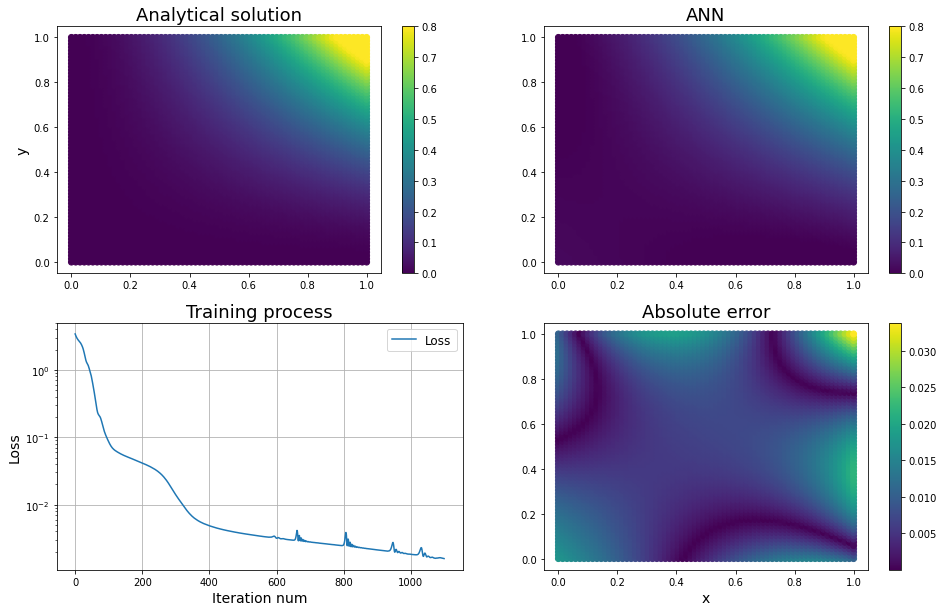
\includegraphics[width=\textwidth]{images/chapter2/pde_1_2.png}
	\caption{Solution of equation 2 from the table \ref{table:pde1_tab}}
	\label{fig:pde_1_2}
\end{figure}

\begin{table}
	\centering
	\begin{tabular}{| c | c | c | c | c |} 
		\hline
		$f(x) = $ & Solution & Equation number & Solution accuracy & Figure \\ \hline
		$ -2 sin(x) cos(y) $ & $ y = sin(x) cos(y) $ & 1 & 6.0114e-06 & \ref{fig:pde_1_1} \\
		$ 2 y^2 + 2 x^2 $ & $ y = x^2 y^2 $ & 2 & 7.1142e-05 & \ref{fig:pde_1_2}  \\ \hline
	\end{tabular}
	\caption{Results for the equations from the table \ref{table:pde1_tab}}
	\label{table:pde1_tab_results}
\end{table}

In table \ref{table:pde1_tab_results}, the accuracy column reflects the average normalized root of the deviation, or in other words, the average deviation from the analytical solution. The figures show that the solution built by the neural network is close to true, and also reflects all the features of the function. The convergence on the graphs without problems and jumps between local extremes, which is good. In general, to solve the specifically given equation, the method is suitable for any other too, but it may require adjustment of the network architecture, the choice of an optimizer and the duration of the training.
\section*{Conclusions}
In this chapter, approximation problems based on linear regression were considered. For linear regression, basic methods for estimating coefficients were considered, and problems that may arise in the process of their estimation were also considered, such as insufficiently generalized ability due to lack of data or strong collinearity of data, leading to a high value of the condition number. Then, from the basic task of supervised learning, a transition was made to replacing the kernel in linear regression and possible replacements, such as the transformation of linear regression into the restoration of the image of the function in the Fourier and Chebyshev space, were considered. Specifically, these functions were considered in view of the fact that there are strong theorems guaranteeing convergence in pointwise and in the sense of the $L_2$ norm. Also, theorems on decreasing coefficients cannot be left unnoticed, since without loss of quality it is possible to limit these expansions in the future and not worry about subsequent effects. After the conclusions made that in the general case, with an arbitrary core, the linear regression model only builds an expansion in basic functions, it was suggested that a single-layer neural network is a similar expansion, with a pre-selected core - a sigmoid function. For this function, there is Tsybenko’s theorem guaranteeing the quality of approximation of arbitrary accuracy with an increase in the number of terms in the expansion. All these conclusions lead to the conclusion that to solve differential equations it remains only to correctly compose the optimization problem, then the solution will be guaranteed to be found, if it exists for the initial problem itself. Ideas and conclusions were borrowed from various works, and are indicated in the list of sources. However, it is worth noting that no work with a similar approach has been encountered before and this issue will be further worked out. In addition it is worth noting the second fact that the current chapter fully explains that to solve differential equations by the method using neural networks, it is enough to use single-layer networks, which significantly narrows the family of architectures for learning. An increase in depth is guaranteed to lead to an improvement in the solution with sufficient training time, however, effects appear associated with jumps in the objective function during training process due to the large number of local minima. For the tasks, we used the same optimization algorithm based on gradient descent and the influence of the algorithm parameters, as well as the choice of the algorithm itself on the quality of the solution and the rate of convergence, was not investigated, but most likely the results will differ and still this is important. At the end, solutions of typical problems for ODEs, system of ODE, and a one-dimensional partial differential equation were presented. Partial differential equations systems are presented in a next  chapter, since in addition to the introduced criteria for training a neural network, an important feature of the work is the solution of partial differential equations systems.
